\documentclass[11pt]{article}

% \textbf{
% Introduction to Programming the Robot Car’s TMS320F28379D Processor. \\
% One-Week Lab
% }

\def\AssignmentMode{Lab}     % HW | Lab | LabVIEW
\def\HWNum{3}
\def\AssignmentText{Introduction to Programming the Robot Car’s TMS320F28379D Processor. \\
One-Week Lab}

% Course metadata
% ============================
% Required packages
% ============================

% \usepackage[letterpaper, total={6in, 9.5in}]{geometry}
\usepackage[
  letterpaper,
  left=0.5in,
  right=0.5in,
  top=0.5in,
  bottom=1.0in
]{geometry}


\usepackage[most]{tcolorbox}
\usepackage{booktabs}
\usepackage{fancyhdr}
\usepackage{graphicx}
\usepackage[
  colorlinks=true,
  linkcolor=blue,
  urlcolor=blue,
  citecolor=blue
]{hyperref}
\usepackage{lastpage}
\usepackage{listings}
\usepackage{minted}
\usepackage{setspace}
\usepackage{subcaption}
\usepackage{tabularx}
\usepackage{tikz}
\usepackage{xcolor}
\usepackage{xparse}
\usepackage[siunitx, american, RPvoltages]{circuitikz}
% Required packages:
\usepackage[table]{xcolor}
\usepackage{array}
\usepackage{array,colortbl,xcolor}
\usepackage{pdflscape}
\usepackage{pgfplots}
\usepackage{xurl}
\usetikzlibrary{arrows.meta, angles, quotes, shapes.symbols, arrows.meta}


\usepackage{pgfcalendar}

%%%%%%%%%%%%%%%%%%%% MODIFY DATES HERE %%%%%%%%%%%%%%%%

\def\Year{2026}
\def\StartDate{\Year-01-19}

\def\HWCheckOffTime{5PM}
\def\HWSubmitTime{9AM}
\def\LabVIEWSubmitTime{5PM}

%%%%%%%%%%%%%%%%%%%%%%%%%%%%%%%%%%%%%%%%%%%%%%%%%%%%%%%

\newcount\julianday
\newcount\myweekday % Define a counter for the weekday index

\newcommand{\GetDate}[2]{%
    \pgfcalendardatetojulian{\StartDate}{\julianday}%
    \advance\julianday by \numexpr #1*7 + #2\relax%
    % 1. Convert JDN to a date (sets \myyear, \mymonth, \myday)
    \pgfcalendarjuliantodate{\julianday}{\myyear}{\mymonth}{\myday}%
    % 2. Convert JDN to a weekday index 0..6 and store in \myweekday
    \pgfcalendarjuliantoweekday{\julianday}{\myweekday}%
    % 3. Print the name using the index, then the rest
    \pgfcalendarweekdayname{\myweekday}, \pgfcalendarmonthname{\mymonth} \myday%
}

\def\Final{\GetDate{16}{3}}
\usepackage{tikz}
\usepackage{xcolor}

\definecolor{iconGold}{RGB}{249,219,132}
\definecolor{iconGreen}{RGB}{71,160,93}

% Derived Border Colors (Darkened for contrast)
\definecolor{borderGold}{RGB}{180,150,80}
\definecolor{borderGreen}{RGB}{50,110,65}

\tikzset{
    ide_icon/.style={
        baseline=-0.3ex,
        line join=round,
        line cap=round,
        % Set a default border width that scales 
        line width=0.4pt 
    }
}

\newcommand{\pauseBtn}[1][0.4]{%
\begin{tikzpicture}[ide_icon, scale=#1]
    \filldraw[fill=iconGold, draw=borderGold] (0,0) rectangle (0.25, 0.8);
    \filldraw[fill=iconGold, draw=borderGold] (0.4,0) rectangle (0.65, 0.8);
\end{tikzpicture}}

\newcommand{\playBtn}[1][0.4]{%
\begin{tikzpicture}[ide_icon, scale=#1]
    \filldraw[fill=iconGold, draw=borderGold] (0,0) rectangle (0.15, 0.8);
    \filldraw[fill=iconGreen, draw=borderGreen] (0.25,0) -- (0.25,0.8) -- (0.75,0.4) -- cycle;
\end{tikzpicture}}

\newcommand{\debugBtn}[1][0.55]{%
\begin{tikzpicture}[ide_icon, scale=#1, rotate=45]
    % Legs: use border color for the stroke
    \draw[borderGreen, line width=0.6pt] (-0.3, 0.5) -- (0.3, 0.1);
    \draw[borderGreen, line width=0.6pt] (-0.3, 0.3) -- (0.3, 0.3);
    \draw[borderGreen, line width=0.6pt] (-0.3, 0.1) -- (0.3, 0.5);

    % Antenna
    \draw[borderGreen, line width=0.6pt] (0, 0.6) -- (-0.15, 0.75);
    \draw[borderGreen, line width=0.6pt] (0, 0.6) -- (0.15, 0.75);
    % Body
    \filldraw[fill=iconGreen, draw=borderGreen] (0,0.3) ellipse (0.18 and 0.25);
    % Head
    \filldraw[fill=iconGreen, draw=borderGreen] (0,0.6) circle (0.08);

\end{tikzpicture}}

\newcommand{\restartBtn}[1][0.8]{%
\begin{tikzpicture}[ide_icon, scale=#1]

    % Shaft with border
    \draw[borderGold, line width=1.8pt]
        (0,0.2) -- (0,0) -- (0.4,0) -- (0.4,0.2);

    \draw[iconGold, line width=1.0pt]
        (0,0.2) -- (0,0) -- (0.4,0) -- (0.4,0.2);

    % Arrowhead with proper outline
    \filldraw[
        fill=iconGold,
        draw=borderGold,
        line join=round
    ]
        (-0.1,0.2) -- (0.1,0.2) -- (0,0.33) -- cycle;

    % Green triangle cap
    \filldraw[fill=iconGreen, draw=borderGreen]
        (0.15,0.1) -- (0.15,0.5) -- (0.4,0.3) -- cycle;

\end{tikzpicture}%
}

% ============================
% Assignment mode resolution
% ============================

\def\CourseCode{SE 423}
\def\CourseName{Mechatronics}

\def\AssignmentType{}
\def\AssignmentFooter{}

\makeatletter
\@namedef{Assignment@HW@type}{Homework Assignment}
\@namedef{Assignment@HW@footer}{HW}

\@namedef{Assignment@Lab@type}{Laboratory Assignment}
\@namedef{Assignment@Lab@footer}{Lab}

\@namedef{Assignment@LabVIEW@type}{LabVIEW Assignment}
\@namedef{Assignment@LabVIEW@footer}{LabVIEW}

\@ifundefined{Assignment@\AssignmentMode @type}{
  \PackageError{AssignmentMode}{Invalid AssignmentMode}{%
    Valid options: HW, Lab, LabVIEW}
}{
  \edef\AssignmentType{\@nameuse{Assignment@\AssignmentMode @type}}
  \edef\AssignmentFooter{\@nameuse{Assignment@\AssignmentMode @footer}}
}
\makeatother

% ============================
% Header / footer
% ============================

\pagestyle{fancy}
\fancyhf{}
\fancyfoot[L]{// \CourseCode, \CourseName}
\fancyfoot[R]{// \AssignmentFooter~\HWNum, Page \thepage\ of \pageref{LastPage}}
\renewcommand{\headrulewidth}{0pt}

% ============================
% Title box
% ============================

\newcommand{\MakeAssignmentTitle}{
\begin{tcolorbox}[
    colback=gray!30!white,
    width=\textwidth,
    boxrule=0.8pt,
    arc=2mm,
    left=6mm,
    right=6mm,
    top=4mm,
    bottom=4mm,
    center
]
\centering
\setstretch{1.2}

\textbf{\Large \CourseCode\ \CourseName \\ \AssignmentType\ \#\HWNum}

\vspace{2mm}

\textbf{
\AssignmentText
}
\end{tcolorbox}
\vspace{0.5cm}
}

\setmintedinline{breaklines, breakafter=_}


\setminted{
  breaklines,
  breakanywhere=false,
  breakafter=\space,
  frame=lines,
  fontsize=\footnotesize,
}


\lstset{
    basicstyle=\ttfamily,   % Typewriter font for code
    breaklines=true,        % Allow breaking long lines
    columns=flexible        % Makes spacing better for inline
}

\newcounter{exercise}

\NewDocumentCommand{\Ex}{o}{
  \stepcounter{exercise}
  \section*{Exercise \theexercise
    \IfValueT{#1}{: #1} 
  }
  \addcontentsline{toc}{section}{Exercise \theexercise
    \IfValueT{#1}{: #1}}
}


\newcolumntype{C}[1]{>{\centering\arraybackslash}p{#1}}

\pgfplotsset{compat=1.18} 
%
\begin{document}

\MakeAssignmentTitle

\section*{Goal for this Lab Assignment}
%
\begin{enumerate}
\item Understand how a duty cycle varying square wave (PWM) can be used to command a seemingly linear and analog output.
\item Use EPWM12A to control the brightness of LED1.
\item Use EPWM1A and EPWM2A to command your robot’s two DC motors in both the clockwise and counter-clockwise direction. Create two functions, \mintinline{c}{setEPWM1A} and \mintinline{c}{setEPWM2A}, that will help you prepare to control the motor's speed and angle in future labs.
\item Use EQEP1, EQEP2 to read the angle movement in motor 1 and in motor 2. Calculate the spin rate of each wheel. Use EQEP3 as a command input to the robot.  
\item Sample the robot moving at different speeds and plot the friction curves for your robot. Then use these friction curves to compensate for the robot's friction.  
\end{enumerate}
%
\begin{center}
\Large
    \textbf{\textcolor{red}{Your robot can only be sitting in two locations: on the floor or on a stand on the bench with all wheels off the bench.}}
\end{center}
%
Failure to do so may result in robot suicide, i.e., the robot may suddenly drive itself off the bench. If a student catastrophically breaks their robot, both the instructor’s and the student’s lab work will triple. Both will still have to come to the lab; both will have to come after lab hours to use another group’s robot to complete the lab; and both will have to come in after hours to repair the robot so it can be used in other lab sections.

\section*{Laboratory Exercises}

\Ex[EPWM Peripheral]

Ask your instructor if there are changes to the repository. If there are, open a terminal and run through the steps in the “Using the SE423 repository” and “Course File Updates” sections. Once you have finished, create a new project from LABstarter as you have in previous labs and rename this project \verb|Lab3<yourinitials>|.

Also, ask your instructor if the PWM from the F28379D board is connected to the robot’s motor amplifiers. \textit{This is a note to the instructor to check if the PWM cable has been moved from connecting to the F28027 chip to the F28379D board. This would only be the case if we forgot to move the cable after the previous semester.}  

As discussed in the lecture, the EPWM peripheral has many more options than we will need for SE423 this semester. We only need to focus on the peripheral's basic features. I have created a condensed version of the EPWM chapter of the F28379D technical reference guide. The condensed version can be found here \url{http://coecsl.ece.illinois.edu/SE423/EPWM_Peripheral.pdf}. The complete technical reference guide can be found here \url{http://coecsl.ece.illinois.edu/SE423/tms320f28379D_TechRefi.pdf}.   

To set up the PWM peripheral and its output channels, you will need to program the PWM peripheral registers through the “bit-field” unions TI defined. Let us look at the bit-field definitions for the registers TBCTL and AQCTLA. (Note: you can find these definitions in Code Composer Studio also by typing in the text EPwm12Regs, somewhere in your \mintinline{c}{main()} function, and then right clicking and selecting “Open Declaration.”  Then do that one more time on the \mintinline{c}{TBCTL_REG} union. \textbf{YOU DO NOT} cut and paste the below code into your code. I am just showing you how to view variable definitions using the “Open Declaration” command. Make sure to delete this single line of code where you typed \mintinline{c}{EPwm12Regs}, otherwise you will receive a compiler error later.)
%
\begin{minted}{c}
struct TBCTL_BITS {                     // bits description
    Uint16 CTRMODE:2;                   // 1:0 Counter Mode
    Uint16 PHSEN:1;                     // 2 Phase Load Enable
    Uint16 PRDLD:1;                     // 3 Active Period Load
    Uint16 SYNCOSEL:2;                  // 5:4 Sync Output Select
    Uint16 SWFSYNC:1;                   // 6 Software Force Sync Pulse
    Uint16 HSPCLKDIV:3;                 // 9:7 High Speed TBCLK Pre-scaler
    Uint16 CLKDIV:3;                    // 12:10 Time Base Clock Pre-scaler
    Uint16 PHSDIR:1;                    // 13 Phase Direction Bit
    Uint16 FREE_SOFT:2;                 // 15:14 Emulation Mode Bits
};

union TBCTL_REG {
    Uint16 all;
    struct TBCTL_BITS bit;
};
struct AQCTLA_BITS {                    // bits description
    Uint16 ZRO:2;                       // 1:0 Action Counter = Zero
    Uint16 PRD:2;                       // 3:2 Action Counter = Period
    Uint16 CAU:2;                       // 5:4 Action Counter = Compare A Up
    Uint16 CAD:2;                       // 7:6 Action Counter = Compare A Down
    Uint16 CBU:2;                       // 9:8 Action Counter = Compare B Up
    Uint16 CBD:2;                       // 11:10 Action Counter = Compare B Down
    Uint16 rsvd1:4;                     // 15:12 Reserved
};

union AQCTLA_REG {
    Uint16 all;
    struct AQCTLA_BITS bit;
};
\end{minted}
%
Looking at these bit-fields notice the \mintinline{c}{:1}, \mintinline{c}{:2} or \mintinline{c}{:3} after \mintinline{c}{PHSEN}, \mintinline{c}{CTRMODE}, \mintinline{c}{CLKDIV} respectively. This tells how many bits this portion of the bit-field uses. If you add up all the numbers after the colons, you see that it adds to 16, which is the size of both the \mintinline{c}{TBCTL} and \mintinline{c}{AQCTLA} registers. So each bit of the register can be assigned by this bit-field. To make this clearer, look at the definition of \mintinline{c}{TBCTL} and \mintinline{c}{AQCTLA} from TI’s technical reference guide:
%
\begin{table}[H]
\caption{TBCTL Register: Figure 15-93}
\footnotesize
\centering
% \renewcommand{\arraystretch}{1.4}
% \setlength{\tabcolsep}{4pt}
\setlength{\tabcolsep}{0pt} % eliminate horizontal padding

% Color definitions (matched to figure)
\definecolor{bitbg}{RGB}{255,255,210}    % lighter yellow
%
\begin{tabular}{|*{8}{C{2cm}|}}

\hline

\rowcolor{bitbg}
15 & 14 & 13 & 12 & 11 & 10 & 9 & 8 \\
\hline

\multicolumn{2}{|c|}{FREE\_SOFT} &
\multicolumn{1}{c|}{PHSDIR} &
\multicolumn{3}{c|}{CLKDIV} &
\multicolumn{2}{c|}{HSPCLKDIV} \\
\hline

\multicolumn{2}{|c}{R/W-0h} &
\multicolumn{1}{c}{R/W-0h} &
\multicolumn{3}{c}{R/W-0h} &
\multicolumn{2}{c|}{R/W-1h} \\
\hline

\rowcolor{bitbg}
7 & 6 & 5 & 4 & 3 & 2 & 1 & 0 \\
\hline

\multicolumn{1}{|c|}{HSPCLKDIV} &
\multicolumn{1}{c|}{SWFSYNC} &
\multicolumn{2}{c|}{SYNCOSEL} &
\multicolumn{1}{c|}{PRDLD} &
\multicolumn{1}{c|}{PHSEN} &
\multicolumn{2}{c|}{CTRMODE} \\
\hline

\multicolumn{1}{|c|}{R/W-1h} &
\multicolumn{1}{c}{R-0/W1S-0h} &
\multicolumn{2}{c}{R/W-0h} &
\multicolumn{1}{c}{R/W-0h} &
\multicolumn{1}{c}{R/W-0h} &
\multicolumn{2}{c|}{R/W-3h} \\
\hline

\end{tabular}
\end{table}
%
and
%
\begin{table}[H]
\caption{AQCTLA Register: Figure 15-115}
\footnotesize
\centering
% \renewcommand{\arraystretch}{1.4}
% \setlength{\tabcolsep}{4pt}
\setlength{\tabcolsep}{0pt} % eliminate horizontal padding

% Color definitions (matched to figure)
\definecolor{bitbg}{RGB}{255,255,210}    % lighter yellow
%
\begin{tabular}{|*{8}{C{1.85cm}|}}

\hline

\rowcolor{bitbg}
15 & 14 & 13 & 12 & 11 & 10 & 9 & 8 \\
\hline


\multicolumn{4}{|c|}{\cellcolor{gray!30}RESERVED} &
\multicolumn{2}{c|}{CBD} &
\multicolumn{2}{c|}{CBU}  \\
\hline

\multicolumn{4}{|c}{R-0-0h} &
\multicolumn{2}{c}{R/W-0h} &
\multicolumn{2}{c|}{R/W-0h} \\
\hline

\rowcolor{bitbg}
7 & 6 & 5 & 4 & 3 & 2 & 1 & 0 \\
\hline

\multicolumn{2}{|c|}{CAD} &
\multicolumn{2}{c|}{CAU} &
\multicolumn{2}{c|}{PRD} &
\multicolumn{2}{c|}{ZRO} \\
\hline

\multicolumn{2}{|c}{R/W-0h} &
\multicolumn{2}{c}{R/W-0h} &
\multicolumn{2}{c}{R/W-0h} &
\multicolumn{2}{c|}{R/W-0h} \\
\hline

\end{tabular}
\end{table}
%
Notice that CLKDIV occupies 3 bits of the TBCTL register. CAU takes up 2 bits of the AQCTLA register. What bit-field unions allow us to do in our program is assign the value of the three CLKDIV bits without changing the other bits of the register. So you could code:
%
\begin{minted}{c}
EPwm12Regs.TBCTL.bit.CLKDIV = 3;
\end{minted}
%
Moreover, that would set bit 10 to \verb|1|, bit 11 to \verb|1|, and bit 12 to \verb|0| in the TBCTL register and leave all the other bits the way they were. Since CLKDIV uses 3 bits, the smallest value you can set it to is 0. \textbf{What is the largest number you could set it to?}  (\textit{Technically, you could set it to any number, but only the bottom 3 bits of the number are looked at in the assignment}.)  \textbf{For the bit-field section CAU in AQCTLA, what are the numbers it can be assigned to?}  Looking at the \href{http://coecsl.ece.illinois.edu/SE423/EPWM_Peripheral.pdf}{condensed Tech. Ref.}, \textbf{how do these different values assigned to AQCTLA’s CAU section change the PWM output? Show these answers to your TA.}

So, given that introduction to register bit-field assignments, let us write some code in our \mintinline{c}{main()} function to set up EPWM12A to drive LED1. \textit{If I do not list an option that you see defined in a register, then that means you should not set that option, and it will be kept as the default. I may suggest an option that is already the default, but to make it clear to the reader of your code that this option is set, I would like you to assign it the default value, even though that line of code is not necessary.}   Set the following options in the EPWM registers for EPWM12A. A good place to write this initialization code is in your \mintinline{c}{main()} function, right after the calls to \mintinline{c}{init_serialSCI{A, B, C, D}()}  (Leave C and D commented out). Most of your initializations should be placed there.

With TBCTL, write four lines of code to set: Count up Mode, Free Soft emulation mode to Free Run so that the PWM continues when you set a break point in your code, disable the phase loading, and Clock divide by 1. 

With TBCTR: Start the timer at zero.

With TBPRD, set the PWM signal period (carrier frequency) to 20 kHz, corresponding to a period of 50 microseconds. Remember, the clock source the TBCTR register is counting has a frequency of 50 MHz, or a period of 1/50000000 seconds.  

With CMPA, initially start the duty cycle at 50\%.  

With AQCTLA set, set the PWM signal to clear when CMPA is reached, and set the pin when the TBCTR register is zero.  

With TBPHS set to zero, i.e., \mintinline{c}{EPwm12Regs.TBPHS.bit.TBPHS =0;}  I do not know if this setting is necessary, but I have seen it in several TI examples, so I am just being safe here.  

You also need to set the PinMux so EPWM12A is used instead of GPIO22. Use the \href{http://coecsl.ece.illinois.edu/SE423/Lab_PinMuxTableF28379DLaunchPadSE423Robot.pdf}{PinMux table for the F28379D Launchpad} to help you here. Use the function \mintinline{c}{GPIO_SetupPinMux} to change the PinMux such that GPIO22 is instead set as EPWM12A output pin. For example, the below line of code sets GPIO158 as GPIO158: 
%
\begin{minted}{c}
GPIO_SetupPinMux(158, GPIO_MUX_CPU1, 0); //GPIO PinName, CPU, Mux Index
\end{minted}
%
Looking at the PinMux table, the following line of code sets GPIO40 to be instead the SDAB pin:
%
\begin{minted}{c}
GPIO_SetupPinMux(40, GPIO_MUX_CPU1, 6); //GPIO PinName, CPU, Mux Index  
\end{minted}
%
Finally, based on several TI examples, it seems a good idea to disable the pull-up resistor when an I/O pin is set as a PWM output to reduce power consumption. Add these five lines of code in the same area of your \mintinline{c}{main()} function. You will be setting up EPWM1A and EPWM2A later in this lab. I went ahead and added their code here to simplify the explanation of the later steps in the lab. 
%
\begin{minted}{c}
EALLOW;  // Below are protected registers
GpioCtrlRegs.GPAPUD.bit.GPIO0 = 1; // For EPWM1A
GpioCtrlRegs.GPAPUD.bit.GPIO2 = 1; // For EPWMA2
GpioCtrlRegs.GPAPUD.bit.GPIO22 = 1; // For EPWM12A
EDIS;
\end{minted}
%
Compile your code and fix any compiler errors. When ready, download this code to your Launchpad. When you run your code, the EPWM12A signal driving LED1 has a 50\% duty cycle, so LED1 should be 50\% on. You will change the duty cycle of EPWM12A by manually updating its CMPA register in Code Composer Studio. In CCS, select the menu View $rightarrow$ Registers, and the Registers tab should appear. There are a bunch of registers, so you will have to scroll down until you see the “EPwm12Regs” register. Click the “$>$” to expand the register. Scroll down until you find the TBPRD and CMPA registers. Note the value in TBPRD. Expand the CMPA register and confirm that it is a 32-bit register with two 16-bit parts, CMPA and CMPAHR. Leave CMPAHR at 0 and change CMPA. First, try setting CMPA to 3/4th the value of TBPRD. What happens to the intensity of LED1? Change CMPA to the same value as TBPRD to see the maximum brightness (100\% duty cycle). Play with other values for CMPA to see the brightness change. Also, at this time, have your TA show you how to scope this PWM signal driving LED1. \textbf{Always shut down the Raspberry Pi, if it is on (which it should not be for this lab), and power off your Robot when connecting the scope probes. }

Now that you see CMPA changes the brightness of LED1, write code in CPU Timer2’s interrupt function to increase, by one, the value of EPWM12’s CMPA register every one millisecond. Then, when CMPA reaches the value in TBPRD, set your code's state to decrease CMPA by 1 each millisecond; when CMPA reaches 0, start increasing CMPA by 1 again each millisecond. This way, your code will change the duty cycle from 0 to 100, then from 100 to 0, and keep repeating this process. The easiest way to code this is to create a global variable of type \mintinline{c}{int16_t} named updown. When updown is equal to 1, count up; when updown is 0, count down. When counting, check for CMPA to reach the value of TBPRD and switch to down counting. While down-counting, check if CMPA equals zero to switch back to up-counting. \textbf{Demonstrate working code to your TA.}
%
\begin{figure}[H]
    \centering
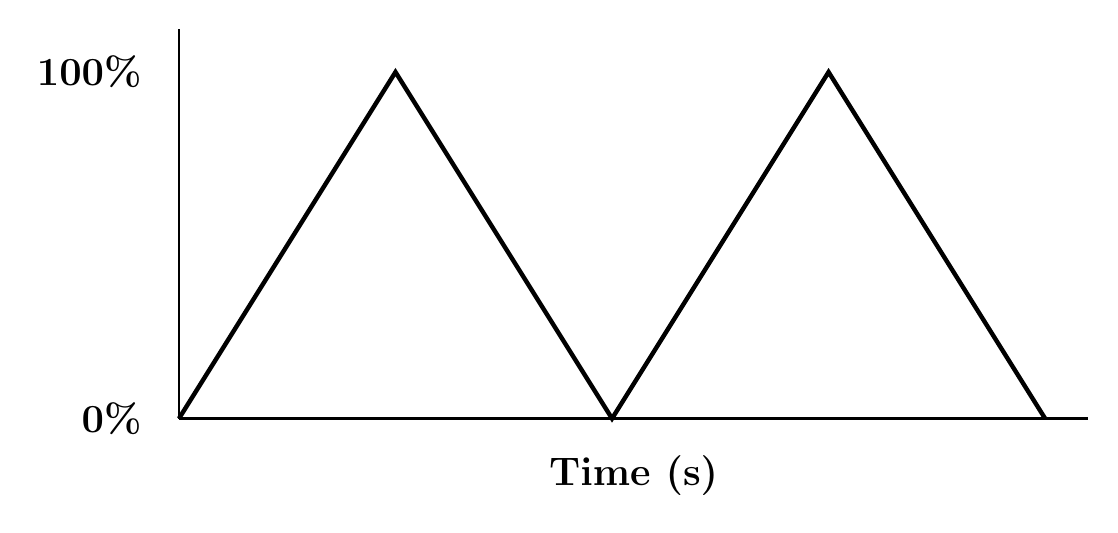
\begin{tikzpicture}[scale=1.1]

    % Axes
    \draw[thick] (0,0) -- (10.5,0); % x-axis
    \draw[thick] (0,0) -- (0,4.5);  % y-axis

    % Axis labels
    \node[below=10pt] at (5.25,0) {\Large\textbf{Time (s)}};
    \node[left=10pt] at (0,0) {\Large\textbf{0\%}};
    \node[left=10pt] at (0,4) {\Large\textbf{100\%}};

    % Triangular waveform
    \draw[ultra thick]
        (0,0) --
        (2.5,4) --
        (5,0) --
        (7.5,4) --
        (10,0);
\end{tikzpicture}
    \caption{Ramped LED1 Brightness Pattern}
    \label{fig:placeholder}
\end{figure}
%
Before proceeding to Exercise 2, let us copy the EPWM12A settings and apply them to EPWM1 and EPWM2. EPWM1A and 2A will be used to drive the robot’s DC motors through an H-bridge IC.  

	Using the \mintinline{c}{GPIO_SetupPinMux} function, set GPIO0’s pin function to EPWM1A, and using another call to \mintinline{c}{GPIO_SetupPinMux}, set GPIO2’s pin function to EPWM2A. Use the \href{http://coecsl.ece.illinois.edu/se423/Lab_PinMuxTableF28379DLaunchPadSE423Robot.pdf}{PinMux Table} to find the correct mux setting.     
    
Compile and debug your code to ensure you did not introduce any typos. All we did was add some additional initializations, so your code should work the same.   

\Ex[EPWM to drive Robot’s DC Motors]

Very similar to the start of Exercise 1, please play with the EPWM1A and EPWM2A registers in the CCS Registers window to make both motors spin at different speeds and change their directions. EPWM1A (GPIO0) controls the left motor. EPWM2A (GPIO2) controls the right motor. From the lecture, you should remember that each of these PWM signals drives the “Direction” pin of the motor’s amplifier (H-bridge). That means if we command a 50\% duty cycle, the motor is told to spin in the positive direction 50\% of the time and the negative direction 50\% of the time. Because the PWM carrier frequency is high-speed, 20Khz, the motor will see that signal as a zero input, and the motor will not move. 100\% duty cycle will drive the motor with full torque in the positive direction. 0\% duty cycle will drive the motor with full torque in the negative direction. For example, a 75\% duty cycle would drive the motor in the positive direction at 50\% of full torque. Try a few duty cycles and make sure to switch the direction of both motors. \textbf{Demonstrate to your TA.}

Create two functions “\mintinline{c}{void setEPWM1A(float controleffort)}” and “\mintinline{c}{void setEPWM2A(float controleffort)}” that take as a parameter a floating point value “\mintinline{c}{controleffort}”. Both of these functions will set EPWM1A or EPWM2A to a PWM duty cycle value related to the passed “\mintinline{c}{controleffort}” value. When I design/code a digital controller, I always think of my control output (or control effort) to the system I am controlling as a value between -10 and 10. This is just the range I (and others) have chosen. I have seen other research papers and textbooks use ranges like -1 to 1, -100 to 100, 0 to 200, etc. By keeping the same range of output in all my controller designs, I can usually guess at good “ballpark” starting values for my controller gains, like $K_P$, $K_I$, and $K_D$ in a PID controller. Perform the following steps/code in each of these functions:
%
\begin{enumerate}
\item For the \mintinline{c}{float} “\mintinline{c}{controleffort}” function parameter, I would like you to use the range of -10 to 10. To make sure nothing greater than this function uses this range, use two if statements inside your functions to saturate \mintinline{c}{controleffort}. If the value passed is greater than 10, set it to 10. If the value passed is less than -10, set it to -10.    
\item Determine the value to set in CMPA for EPWM1A and CMPA for EPWM2A. Remember that a duty cycle of 50\% is a command of zero to the motor. Any duty cycle greater than 50\% will cause the motor to spin in the positive direction. Any duty cycle less than 50\% will cause the motor to spin in the negative direction. In your functions, linearly scale the control effort, which is in the range -10 to 10, to a duty cycle where -10 is 0\% duty cycle, 0 is 50\%, and 10 is 100\%. Given the duty cycle in this linear scaling, set CMPA to the corresponding percentage. There is an issue with type conversions here. I asked you to make “\mintinline{c}{controleffort}” a float, but CMPA is a 16-bit integer. The good news is that C does much of the type conversion for you automatically. Let us say that the scaled value you would like to set CMPA to is 345.67, stored in the variable \mintinline{c}{float mytmp}. If you perform the C instruction “\mintinline{c}{CMPA = mytmp}”, the value will be truncated, and CMPA will be assigned 345. It will NOT be rounded up to 346. Also, keep in mind that an integer divided by an integer gives you back an integer. For example, this statement “float value = 1/5000” is always 0. You would need to change the line to “float value = 1.0/5000.0” to assign the fraction to value. Also, if you have two \mintinline{c}{int16_t} variables and you divide them, the result is an integer (\mintinline{c}{int16_t}). If you want to assign a \mintinline{c}{float} the division of two integers, you have to type cast the integers to a \mintinline{c}{float}, i.e., “\mintinline{c}{value = ((float)myint1)/((float)myint2)}.”
\item In the same fashion you did in exercise 1 and using the functions you just created, gradually increase the command to the motor until you get to 10, and then gradually decrease the motor command until -10 is reached, and then repeat. Here, you will not increment the CMPA value directly or check whether \mintinline{c}{CMPA==TBPRD}, but instead add to the float value you are passing to your \mintinline{c}{setEPWM} functions. Every 1ms, add 0.005 to the values passed to \mintinline{c}{setEPWM} until 10 is reached, then start subtracting 0.005 from the values until -10 is reached, and repeat. \textbf{Show your TA that your setEPWM functions are working correctly.}      
\end{enumerate}
%
\Ex[EQEP Peripheral, Optical Encoders to find angle of the robot’s wheels and the robot’s speed]

The eQEP peripheral, right out of a “power on reset” of the F28379D processor, is pretty much ready to count the A and B channels of an encoder angle sensor. For that reason, I am providing the code to initialize and read the angle values. The eQEP module has many advanced features, and I have not had a chance to play with many of them yet. If this sounds interesting to you, you could turn playing with the advanced features of the eQEP into a part of your final project for this class. The only thing you need to add to the code below is a scale factor that converts the eQEP count value to a wheel angle in radians.  

Look at your robot’s motors. Notice that there is a gear head between the motor and the wheel’s shaft. This gear ratio is 20:1, meaning 20 rotations of the DC motor result in one rotation of the wheel. Also, look at the back end of the robot’s motor and see the enclosed optical encoder. This optical encoder has 500 slits for one rotation of the DC motor. So, one rotation of the motor produces 500 square-wave periods in both the A and B channels. Since the eQEP counts these pulses in quadrature count mode, the total number of counts per revolution of the motor is 4 × 500, or 2000 counts per revolution. \textit{See my current lectures if you are not familiar with the A and B channels and quadrature count mode.}  Then combining this with the gear ratio of the motor, you can calculate the multiplication factor that converts eQEP counts to the number of radians the wheel has turned. Add this to both the \mintinline{c}{ReadEncLeft()} and \mintinline{c}{ReadEncRight()} functions so that they return radians of the wheel. After adding this multiplication factor, paste the code below into your C file. Make sure to define these four functions in advance. Note that the “\mintinline{c}{readEncWheel}” function reads a third optical encoder that you will hold in your hand to command the robot to move forward and backward. I gave you the scale factor for that encoder.  
%
\begin{minted}{c}
void init_eQEPs(void) {

    // setup eQEP1 pins for input
    EALLOW;
    //Disable internal pull-up for the selected output pins for reduced power consumption
    GpioCtrlRegs.GPAPUD.bit.GPIO20 = 1;    // Disable pull-up on GPIO20 (EQEP1A)
    GpioCtrlRegs.GPAPUD.bit.GPIO21 = 1;    // Disable pull-up on GPIO21 (EQEP1B)
    GpioCtrlRegs.GPAQSEL2.bit.GPIO20 = 2;   // Qual every 6 samples
    GpioCtrlRegs.GPAQSEL2.bit.GPIO21 = 2;   // Qual every 6 samples
    EDIS;
    // This specifies which of the possible GPIO pins will be EQEP1 functional pins.
    // Comment out other unwanted lines.
    GPIO_SetupPinMux(20, GPIO_MUX_CPU1, 1);
    GPIO_SetupPinMux(21, GPIO_MUX_CPU1, 1);
    EQep1Regs.QEPCTL.bit.QPEN = 0;    // make sure eqep in reset
    EQep1Regs.QDECCTL.bit.QSRC = 0;   // Quadrature count mode
    EQep1Regs.QPOSCTL.all = 0x0;      // Disable eQep Position Compare
    EQep1Regs.QCAPCTL.all = 0x0;      // Disable eQep Capture
    EQep1Regs.QEINT.all = 0x0;        // Disable all eQep interrupts
    EQep1Regs.QPOSMAX = 0xFFFFFFFF;   // use full range of the 32-bit count
    EQep1Regs.QEPCTL.bit.FREE_SOFT = 2;  // EQep uneffected by emulation suspend in Code Composer
    EQep1Regs.QPOSCNT = 0;
    EQep1Regs.QEPCTL.bit.QPEN = 1;    // Enable EQep

    EALLOW;
    // setup QEP2 pins for input
    //Disable internal pull-up for the selected output pinsfor reduced power consumption
    GpioCtrlRegs.GPBPUD.bit.GPIO54 = 1;    // Disable pull-up on GPIO54 (EQEP2A)
    GpioCtrlRegs.GPBPUD.bit.GPIO55 = 1;    // Disable pull-up on GPIO55 (EQEP2B)
    GpioCtrlRegs.GPBQSEL2.bit.GPIO54 = 2;   // Qual every 6 samples
    GpioCtrlRegs.GPBQSEL2.bit.GPIO55 = 2;   // Qual every 6 samples
    EDIS;
    GPIO_SetupPinMux(54, GPIO_MUX_CPU1, 5); // set GPIO54 and eQep2A
    GPIO_SetupPinMux(55, GPIO_MUX_CPU1, 5); // set GPIO55 and eQep2B
    EQep2Regs.QEPCTL.bit.QPEN = 0;   // make sure qep reset
    EQep2Regs.QDECCTL.bit.QSRC = 0;  // Quadrature count mode
    EQep2Regs.QPOSCTL.all = 0x0;     // Disable eQep Position Compare
    EQep2Regs.QCAPCTL.all = 0x0;     // Disable eQep Capture
    EQep2Regs.QEINT.all = 0x0;       // Disable all eQep interrupts
    EQep2Regs.QPOSMAX = 0xFFFFFFFF;  // use full range of the 32-bit count.
    EQep2Regs.QEPCTL.bit.FREE_SOFT = 2;  // EQep uneffected by emulation suspend
    EQep2Regs.QPOSCNT = 0;
    EQep2Regs.QEPCTL.bit.QPEN = 1;   // Enable EQep

    EALLOW;
    // setup QEP3 pins for input
    //Disable internal pull-up for the selected output pins for reduced power consumption
    GpioCtrlRegs.GPAPUD.bit.GPIO6 = 1;    // Disable pull-up on GPIO54 (EQEP3A)
    GpioCtrlRegs.GPAPUD.bit.GPIO7 = 1;    // Disable pull-up on GPIO55 (EQEP3B)
    GpioCtrlRegs.GPAQSEL1.bit.GPIO6 = 2;   // Qual every 6 samples
    GpioCtrlRegs.GPAQSEL1.bit.GPIO7 = 2;   // Qual every 6 samples
    EDIS;
    GPIO_SetupPinMux(6, GPIO_MUX_CPU1, 5); // set GPIO6 and eQep2A
    GPIO_SetupPinMux(7, GPIO_MUX_CPU1, 5); // set GPIO7 and eQep2B
    EQep3Regs.QEPCTL.bit.QPEN = 0;   // make sure qep reset
    EQep3Regs.QDECCTL.bit.QSRC = 0;  // Quadrature count mode
    EQep3Regs.QPOSCTL.all = 0x0;     // Disable eQep Position Compare
    EQep3Regs.QCAPCTL.all = 0x0;     // Disable eQep Capture
    EQep3Regs.QEINT.all = 0x0;       // Disable all eQep interrupts
    EQep3Regs.QPOSMAX = 0xFFFFFFFF;  // use full range of the 32-bit count.
    EQep3Regs.QEPCTL.bit.FREE_SOFT = 2;  // EQep uneffected by emulation suspend
    EQep3Regs.QPOSCNT = 0;
    EQep3Regs.QEPCTL.bit.QPEN = 1;   // Enable EQep

}

float readEncLeft(void) {
    int32_t raw = 0;
    uint32_t QEP_maxvalue = 0xFFFFFFFFU;  //4294967295U
    raw = EQep1Regs.QPOSCNT;
    if (raw >= QEP_maxvalue/2) raw -= QEP_maxvalue;  // I don't think this is needed and never true
    return (raw*(???));
}

float readEncRight(void) {
    int32_t raw = 0;
    uint32_t QEP_maxvalue = 0xFFFFFFFFU;  //4294967295U  -1 32-bit signed int
    raw = EQep2Regs.QPOSCNT;
    if (raw >= QEP_maxvalue/2) raw -= QEP_maxvalue;  // I don't think this is needed and never true
    return (raw*(???));
}

float readEncWheel(void) {
    int32_t raw = 0;
    uint32_t QEP_maxvalue = 0xFFFFFFFFU;  //4294967295U  -1 32-bit signed int
    raw = EQep3Regs.QPOSCNT;
    if (raw >= QEP_maxvalue/2) raw -= QEP_maxvalue;  // I don't think this is needed and never true
    return (raw*(2*PI/4000.0));
}
\end{minted}
%
Call \mintinline{c}{init_eQEPs()} inside \mintinline{c}{main()} somewhere after the \mintinline{c}{init_serialSCI{A, B, C, D}()} function calls but before the EINT line of code and the \mintinline{c}{while(1)} loop. Then set one of the unused CPU timer interrupts to timeout every 1 millisecond. Inside that CPU timer interrupt function, call the two read functions and assign their return values to float variables like “\mintinline{c}{LeftWheel}” and “\mintinline{c}{RightWheel}”. Your existing code should be setting \mintinline{c}{UARTPrint} to have the \mintinline{c}{main()} while loop print your desired text to the Robot’s text LCD screen. Change the print lines to print your two wheel angle measurements and the third encoder wheel angle. Build and run this code. With your code running, manually move your robot’s wheels. As a check, try rotating one wheel by just one turn. You should see an angle close to $2 \pi$. If not, you have the wrong multiplication factor in your read functions. If the front of the robot car is the side the LIDAR is on and the back is the side the battery is inserted into, does the labeling of the left and right wheels make sense? Forward speed will be defined as the robot's forward motion. As you rotate your wheels, you should see that when you rotate both motors forward, one will give a negative angle. Negate the multiplication factor in that wheel’s read function so that both wheels read a positive angle when rotated in the forward direction. Next, you will be asked to place the robot on the floor and measure how many wheel revolutions it takes to travel 1 foot. Before you do that, you need to program the flash of your F28379D processor so that when you power on your robot, your program runs. So make sure you print both the right- and left-wheel encoder readings to the text LCD screen. Then have your TA show you how to switch to loading your program into the flash of the F28379D processor. Once flashed, unplug the XDS200 JTAG’s USB cable and power off the robot. Then, power back on your robot, and you should see your program running.

Next, in this exercise, you will calculate the speed at which your robot is driving forward or backward. It would be nice to know the robot's speed in ft/s rather than rad/s. Instead of using the wheel's radius, another easy way to convert between radians and feet is to simply put the robot on the floor and move it one or more feet without letting the wheels slip; that will tell you how many radians the wheels turn to cover one foot. Power off your robot, unplug the JTAG, then place the robot on the floor. Line up your robot wheels and push the robot forward 3 feet. Look at the radian values displayed on the robot’s text LCD and divide by 3 feet to find the number of radians per foot. Create two more float variables and store the distance traveled by each wheel using this factor. Print these distances to the robot’s text LCD to check they are correct by pushing the robot a certain distance. \textbf{Does this factor make sense? It should be equal to the radius of the wheel in feet. Show your TA.}  Set the robot back on its stand on the table and reconnect the JTAG.

To finish up this exercise, use the third optical encoder attached to the robot as a type of joystick in your hand to dial in an input to the robot. Perform the following steps within your 0.001-second timer function.  
%
\begin{enumerate}
\item Create two global float variables \mintinline{c}{uLeft},\mintinline{c}{uRight}, to be used as the control outputs to PWM channels 1A and 2A. Modify your previous code so that every 1 ms, the third optical encoder, which you can manually turn, is used to drive the robot’s two motors with the same value. This way, you will have manual control over the robot's forward and backward motion at different speeds. Perform the following:   
\begin{itemize}
\item Set both \mintinline{c}{uLeft} and \mintinline{c}{uRight} equal to \mintinline{c}{Enc3_rad}. NOTE, in later labs \mintinline{c}{uLeft} and \mintinline{c}{uRight} will be assigned values calculated by a control algorithm.
\item Limit \mintinline{c}{uLeft} and \mintinline{c}{uRight} to a value between –10 and 10. 
\item Command EPWM1A and EPWM2A to the value of \mintinline{c}{uLeft} and \mintinline{c}{uRight} using the \mintinline{c}{setEPWM1A} and 2A functions.   
\end{itemize}
\item Using the backwards difference rule (\mintinline{c}{v = (p_current – p_old)/0.001}) as a discrete approximation to the derivative, calculate the linear velocity corresponding to each motor in feet/second from the past and present motor position measurements, \mintinline{c}{p_old} and \mintinline{c}{p_current} respectively.  \mintinline{c}{p_old} is the value of the encoder position 1ms previous.  \textbf{Explain to your TA why }\mintinline{c}{p_old}\textbf{ should be a global variable.}    
\item Print the velocity values of \mintinline{c}{v1} and \mintinline{c}{v2} on the first line of the LCD, and the reading from encoder 3 on the second line of the LCD screen every 100 ms. You have to limit the accuracy of the floating-point numbers you print so all the information fits on the 20-character LCD line. For example, use \%.2f.
\item Make sure that the robot is on the bench stand with wheels OFF the ground. Enable the PWM amplifier when running this code so the motors will spin. The amplifier is enabled by flipping up the switch on the robot’s front amplifier board. When the motors start spinning, check their direction. Given a positive input, both motors should spin to drive the robot forward. \textit{The back end of the robot is the end where the battery can be inserted.} If both the motors do not move in the forward direction when sending a positive control effort, change the sign of the control effort for the motor that is spinning in the wrong direction. The best place to add this negative sign is in front of the parameter passed to the appropriate \mintinline{c}{setEPWM1A} or \mintinline{c}{2A} function. Do not change the sign of the control variable, e.g., if you think motor left is spinning the wrong way given a positive control input, add the sign change to the parameters of \mintinline{c}{setEPWM1A} and do not do something like \mintinline{c}{uLeft = -uLeft;} The sign change is necessary because the motors under the robot are mounted in opposite directions.
\item When you have both motors spinning in the positive direction, given a positive PWM input, check the signs of the two velocity readings. They should both be positive velocities. If you show your TA, it is because you may have performed an earlier step incorrectly. Verify that your velocity (feet/sec) calculation changes if you put a load on the wheels (by adding resistance to the motion with your hand).
\end{enumerate}
%
\Ex[Friction Compensation]

In this final exercise, you are going to implement a friction compensation algorithm to reduce the effects of the motor’s friction on your system. Your task will be to identify the friction acting on the motors. To accomplish this, you will produce a plot of applied motor control effort (or input) (on the y axis) vs. motor velocity (feet/s) (on the x axis). You will first record 10 or so data points, split between positive and negative values. By plotting your data, you can estimate the viscous and Coulomb friction of the motors in both the positive and negative directions.
%
\begin{enumerate}
\item Using the third encoder to change the open-loop command to the motors, record the steady-state ft/sec velocity of the robot driving on the floor at 10 different control inputs. Be sure your measurements make sense… if you read 1 foot per second from the LCD, then the robot should actually be moving approximately 1 foot every second. If the robot is driving too fast to measure the values, you will obviously need to use a smaller control input magnitude. Be sure to measure both positive and negative velocity values (robot moving forward AND backward).
\item Produce a plot of control input vs. speed in MATLAB to \textbf{show to your instructor}.
\item Using two separate regression fits, one for positive velocities and one for negative velocities, find the two lines that best fit your measured data points in the positive and negative velocity regimes. Ask your instructor for help if you do not know how to do a regression in MATLAB quickly. From the best-fit lines, note the y-intercepts. These are your values for positive and negative coulomb friction. We will label these values \verb|Cpos| and \verb|Cneg| (note \verb|Cneg| will be a negative value). The slopes of the two lines are your values for positive and negative viscous friction. We will label these values \verb|Vpos| and \verb|Vneg|.  
\item With these identified parameters, add the following friction compensation algorithm to your code (assuming your motor's one command variable is called “\verb|uLeft|”):
%
\begin{minted}{c}
if (velLeft> 0.0) {
    uLeft = uLeft + Vpos*velLeft + Cpos;
} else {
    uLeft = uLeft + Vneg*velLeft + Cneg;
}
// And perform similar instructions for uRight
\end{minted}
%
As a starting point, use 100\% (in future labs, we will only use 60 - 80\% of the identified values) of the values identified for \verb|Vpos|, \verb|Vneg|, \verb|Cpos|, and \verb|Cneg|. In your code, ensure that only friction compensation is activated for this section. The easiest way to do this is to assign \verb|uLeft| and \verb|uRight| to zero each time in your 1ms code instead of assigning \verb|uLeft| and \verb|uRight| the value of \mintinline{c}{Enc3_rad}. Compile your code.
\end{enumerate}
%
Test your friction compensation code by pushing the robot on the floor. Your robot should roll for a long distance if the friction compensation is working well. You may need to hand-tune your friction gains slightly to get the robot to roll farther when you push it. \textbf{Demonstrate your working code to your instructor.}



\section*{Lab Check Off}
%
\begin{enumerate}
\item Demo Exercise 1, LED getting brighter and dimmer repeatedly.
\item Demo Exercise 2, motors ramping up and down in speed.  
\item Demo Exercise 3, optical encoders working. When spun in the positive direction, both wheel encoders' readings increase.  
\item Demo last part of Exercise 3 using the third encoder to input a control effort to the motors and the robot’s speed displayed to the text LCD screen
\item Demo Exercise 4, your friction plot and your friction compensation working.  
\end{enumerate}
%
\section*{What to Submit to Gradescope}
%
\begin{enumerate}
    \item Your final commented source code for Exercises 1, 2, 3, and 4. Make sure all parts of the exercises are in the code or commented out. Be very clear in your code what parts are for each exercise. Comments should highlight what you learned in this lab.
\end{enumerate}
%
\end{document}